\section{Model Checking the CCUC-protocol}\label{sec:uppaalccuc}
This section will explore to what degree issues caused by unreliability affects the UPPAAL model developed previously in \myref[name]{subsec:changestoModel}.

To do this, every edge which is fired when receiving a message should be changed to have a chance of not receiving anything. 
This can be modeled in UPPAAL SMC using the branch points previously mentioned in \myref[name]{subsec:uppaalsmc}.
This has been done as can be seen on \myref{fig:missTransmission}.

\begin{figure*}[h]
\vspace{-5pt} 
\begin{minipage}{.48\textwidth}
\centering
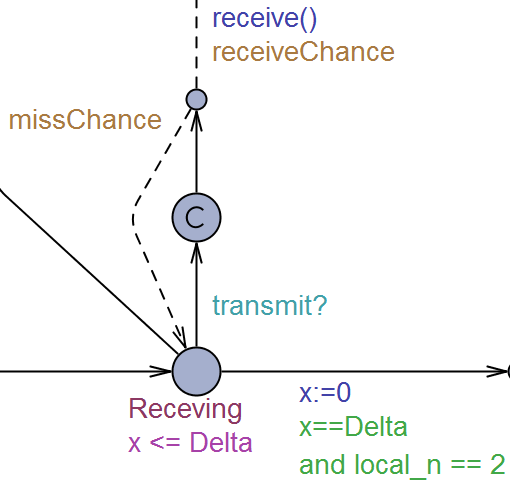
\includegraphics[width=0.7\textwidth]{Figures/Model/MissChance_2.PNG}
\vspace{-10pt} 
\caption{Model in UPPAAL showing the branch node after receiving, where there is a chance for the device to miss the transmission and go back to the previous location.}
\label{fig:missTransmission}
\end{minipage} \hfill
\begin{minipage}{.45\textwidth}
\vspace{82pt}
\begin{lstlisting}[style=UPPAAL, caption={Specifying the reliability of the transmissions, the current numbers result in a 2 \% miss chance.}, label={unreliability-UPPAAL}]
// States how reliable the network is
const int receiveChance = 98;
const int missChance = 100 - receiveChance;
\end{lstlisting}
\end{minipage}
\end{figure*} 

\noindent
The values of \texttt{missChance} and \texttt{receiveChance} are such that their sum is 100, in order to be the same as percentages, their assignments are shown in \myref{unreliability-UPPAAL}.

When the branch points are used everywhere a transmission could be received, the devices will have a miss chance on every transmission received much like in the real world examples, as with the Arduinos and the RF modules used for this project, as found out in \myref[name]{par:wctpl}.
To explore the effect of going from CCRC to CCUC, with the changes to the model mentioned above, the same query from earlier which checks if a network is created can be reused. 
The query is listed in \myref{query-SuccesfulCreate}.

\begin{lstlisting}[style=UPPAAL, caption={Query for UPPAAL which asks for the probability of all devices in a network being equal to the number of devices in the system, and that they all have the same \texttt{network\_id}}, label={query-SuccesfulCreate}]
Pr[<=300000] ( <>  forall(i : id_t) forall(j : id_t) (time > 3000) 
  and ((Device(i).local_n == N+1 
  and Device(i).local_network_id == Device(j).local_network_id)))
\end{lstlisting}

\noindent
With a confidence of 99~\% the probability range lies in the range [0.933723, 0.95372], which means that the somewhere in that range lies the probability of a successful network being created.
This means that the impact of this reliability is actually quite large, and something should be done.
As stated earlier in \myref[name]{sub:avoidance}, one could make the devices transmit more than once in order to reduce the chance of a transmission being completely missed.
To implement this further changes to the model is required.
Therefore the message redundancy technique is implemented in the model, which means that whenever a transmission is sent, it should be able to loop in the same location, transmitting each time, for the number of times it should transmit, before finishing its time-slot. 
This also means that the time-slots' length will have to be increased to make up for the increased transmission time.
One of these loops can be seen on \myref{LoopTransmitUPPAAL}.

\begin{wrapfigure}{r}{0.55\textwidth}
\vspace{12pt}
\centering
  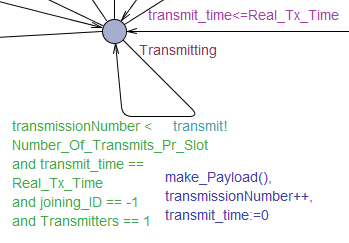
\includegraphics[width=0.55\textwidth]{Figures/Model/Transmit_Loop.PNG} 
\caption{Model in UPPAAL showing the loop, where it transmits for the amount of times specified minus one. The last transmission in a time-slot will occur when it finally leaves the location.}
\label{LoopTransmitUPPAAL}
\end{wrapfigure}

This also requires changes to the code in UPPAAL, which can be found in \myref{UPPAAL-CCUC-Code}.
The complete model for the CCUC-protocol can also be found printed on a piece of A3-paper in the back of the paper.

The model has been tested with the query seen in \myref{query-SuccesfulCreate} with varying miss chance, and with varying number of transmissions in a time-slot.
This should show how the change of transmitting more than once would affect the model.

The results of this test can be seen on \myref{CCUC-Graph-UPPAAL}; they show that transmitting more than once is actually a viable option, as it drastically increases the probability of a network containing all devices will be made, which is close to 99~\% probable whenever transmitting more than once.

A further test has been made to see the changes when the chance of receiving are drastically worse than in the first test.
The result can be seen on \myref{fig:crazy_graph}, where it can be seen just how much it helps transmitting more than once in each time-slot, but it does cost a lot in regards of the speed of the network.

\paragraph{Package Loss in the Main Loop}\hfill \\
The most significant problems regarding the stability of the network occurs when package loss happens during the start-up phase of the network.
However the problems with unreliability lie in the creation of the network, as the model in UPPAAL will work correctly in the main loop.
This was tested by instantiating a network of 4 devices which all started as part of the same network, and had been given different $k$ values, equal to their $id$s
This means that a network is successfully created.
A query was asked to this system, which can be seen on \myref{stable-network-query}.
The results of the query will be a probability in the range [0.980056, 1] with a confidence of 99~\%, which means that the problem truly does lie in connecting to the network, with unreliable transmission. 

\begin{lstlisting}[style=UPPAAL, caption={Query for UPPAAL asking if for all devices i and j, when they are in the location \texttt{User\_Code} will they have they then have the same value for \texttt{local\_i}.}, label={stable-network-query}, float=p]
Pr[<=300000] ( <> forall(i : id_t) forall(j : id_t)  (time > 3000) 
  and  ((Device(i).User_Code and Device(j).User_Code) 
  imply (Device(i).local_i == Device(j).local_i)))
\end{lstlisting} 
 
\begin{figure}[p]
\begin{subfigure}{\linewidth}
\centering
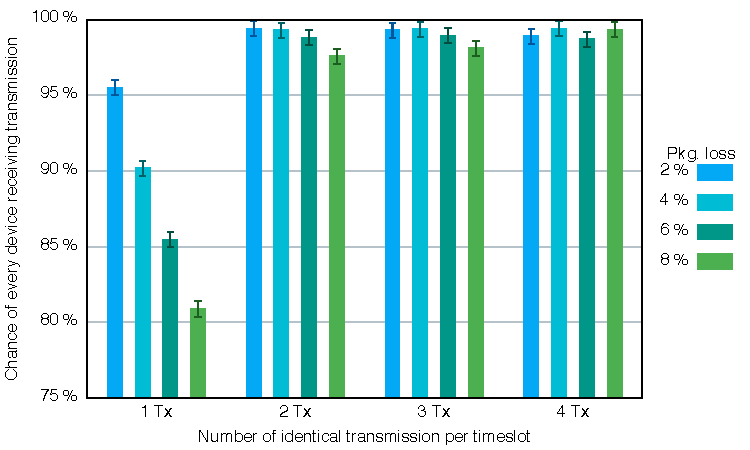
\includegraphics{Figures/Graphs/gnuplot/ccucChance/graph2.pdf} 
\caption{Realistic miss chance}
\label{CCUC-Graph-UPPAAL}
\end{subfigure}\\
\begin{subfigure}{\linewidth}
\centering
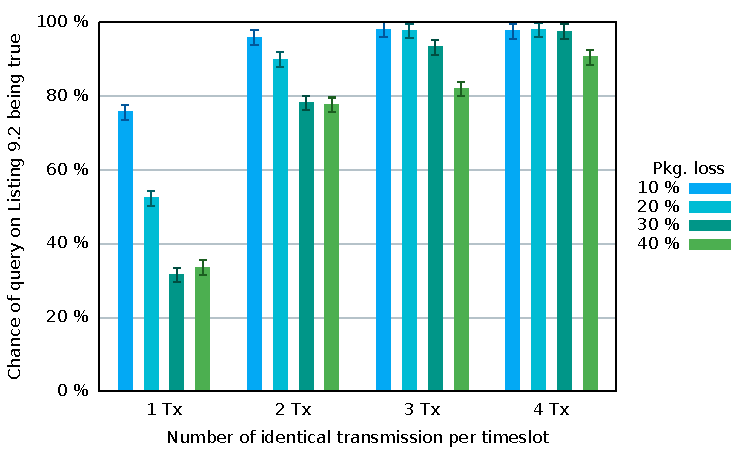
\includegraphics{Figures/Graphs/gnuplot/ccucChance/graph3.pdf} 
\caption{Higher miss chance}
\label{fig:crazy_graph}
\end{subfigure}
\caption{Block-diagrams of the query on \myref{stable-network-query}, with the model that has varying miss chances, using message redundancy.}
\end{figure} 

\paragraph{Conclusion}
Using message redundancy, which is simply transmitting the same message more than once in each time-slot, the probability of a device not receiving a transmission reduces.
Multimessage Echo and the other techniques mentioned in this chapter has not been implemented due to time constraints, and therefore a comparison between the techniques has not been made.
Transmitting more than once in each time-slot will as mentioned reduce the probability of a message not being received, but it does not seem to be a good solution, and also increases the length of the time-slot drastically.
If physical obstacles suddenly stand between two devices it might almost be impossible for the two devices to transmit to each other, and message echoing might have solved this problem.
However two devices having trouble communicating approaches the category of strongly connected networks, which was not the focus of this chapter.